\documentclass[tikz]{standalone}

\usepackage{tikz}



\begin{document}
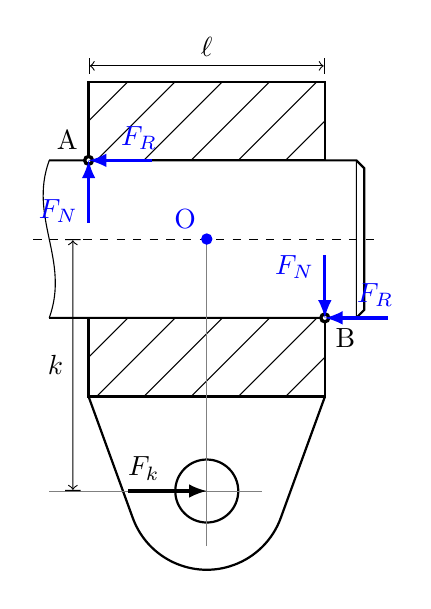
\begin{tikzpicture}

\draw[dashed] (-.2,0)--(4.2,0);
\draw[thick] (0, 1)--(3.9, 1)--(4, .9)--(4, -.9)--(3.9, -1)--(0,-1);
\draw (3.9, 1)--(3.9, -1) (0,1)to[out=250, in=70](0,-1);

\draw[thick] (.5, 1)coordinate(A)rectangle(3.5, 2)coordinate(x);
\begin{scope}
\clip (A)rectangle(x);
\foreach\x in {0,.6,..., 4}{\draw[thin](\x, 1)--++(1,1);}
\end{scope}

\draw[thick] (3.5, -1)coordinate(B)rectangle(.5, -2)coordinate(x);
\begin{scope}
\clip (B)rectangle(x);
\foreach\x in {0,.6,..., 4}{\draw[thin](\x, -2)--++(1,1);}
\end{scope}

\def\len{1.64}
\draw[thick] (x)--++(-70:\len)arc(200:340:1)--++(70:\len);
\draw[thick] (x)++(-70:\len)++(20:1)circle(.4)coordinate(S);


\draw[very thick, fill=white] (A)circle(.05)node[above left]{A};
\draw[very thick, fill=white] (B)circle(.05)node[below right]{B};

\draw[|<->|] (.5, 2.2)--(3.5, 2.2) node[midway, above]{$\ell$};


\draw[help lines] (S)++(.7,0)--++(-2.7,0);
\draw[|<->|] (S)++(-1.7, 0)--(0.3, 0) node[midway, left]{$k$};


\draw[help lines] (S)++(0,-.7)--++(0,3.9)coordinate(O);
\draw[very thick, latex-] (S)--++(-1,0)node[pos=.8, above]{$F_k$};




\draw[very thick, latex-, blue] (A)--++(.8,0)node[pos=.8, above]{$F_R$};
\draw[very thick, latex-, blue] (B)--++(.8,0)node[pos=.8, above]{$F_R$};

\draw[very thick, latex-, blue] (A)--++(0,-.8)node[pos=.8, left]{$F_N$};
\draw[very thick, latex-, blue] (B)--++(0,.8)node[pos=.8, left]{$F_N$};

\draw[very thick, fill=white, blue] (O)circle(.05)node[above left]{O};

\end{tikzpicture}
\end{document}